% O GARCH funcionando em um gráfico (06/11/2026, pedido do autor). NÃO é parte do
% TG. Figura TikZ desta pasta (fig-garch), compilada pelo Makefile, com o
% preâmbulo de ../modelo-completo/comum.tex. Dados e conferência:
% dados/resultados/modelo_completo_2026-11-06/LEIAME.md.
\documentclass[11pt,a4paper]{article}
\usepackage[T1]{fontenc}
\usepackage[brazilian]{babel}
\usepackage{mathptmx}
\usepackage{amsmath}
\usepackage[a4paper,margin=2.2cm]{geometry}
\usepackage{graphicx}
\usepackage[font=small,labelfont=bf]{caption}
\usepackage[most]{tcolorbox}
\usepackage[hidelinks]{hyperref}
\setlength{\parskip}{0.45em}
\setlength{\parindent}{0pt}

\definecolor{cesc}{RGB}{220,50,32}
\definecolor{cmod}{RGB}{0,90,181}
\newtcolorbox{ideia}[1][]{colback=cmod!5, colframe=cmod!70, fonttitle=\bfseries, title={#1}, arc=2pt, boxrule=0.6pt}
\newtcolorbox{cuidado}[1][]{colback=cesc!4, colframe=cesc!70, fonttitle=\bfseries, title={#1}, arc=2pt, boxrule=0.6pt}
\newcommand{\arqm}[1]{../../../dados/resultados/modelo_completo_2026-11-06/#1}
\input{\arqm{valores.tex}}

\title{O GARCH funcionando\\[2pt]\large como um erro do ARIMA vira veto, parcela por parcela}
\author{Material de análise, fora do TG}
\date{6 de novembro de 2026}

\begin{document}
\maketitle

Este relatório mostra o GARCH trabalhando com números reais, num único gráfico de três painéis. O pregão é o
mesmo do relatório \texttt{modelo-completo}, \vSegDia, em que o GARCH vetou uma compra que o ARIMA tinha pedido. A ideia é
mostrar de onde vem a volatilidade prevista, e não só o valor final dela. Nada aqui foi colocado no \texttt{tg/}.

\begin{figure}[h]
\centering
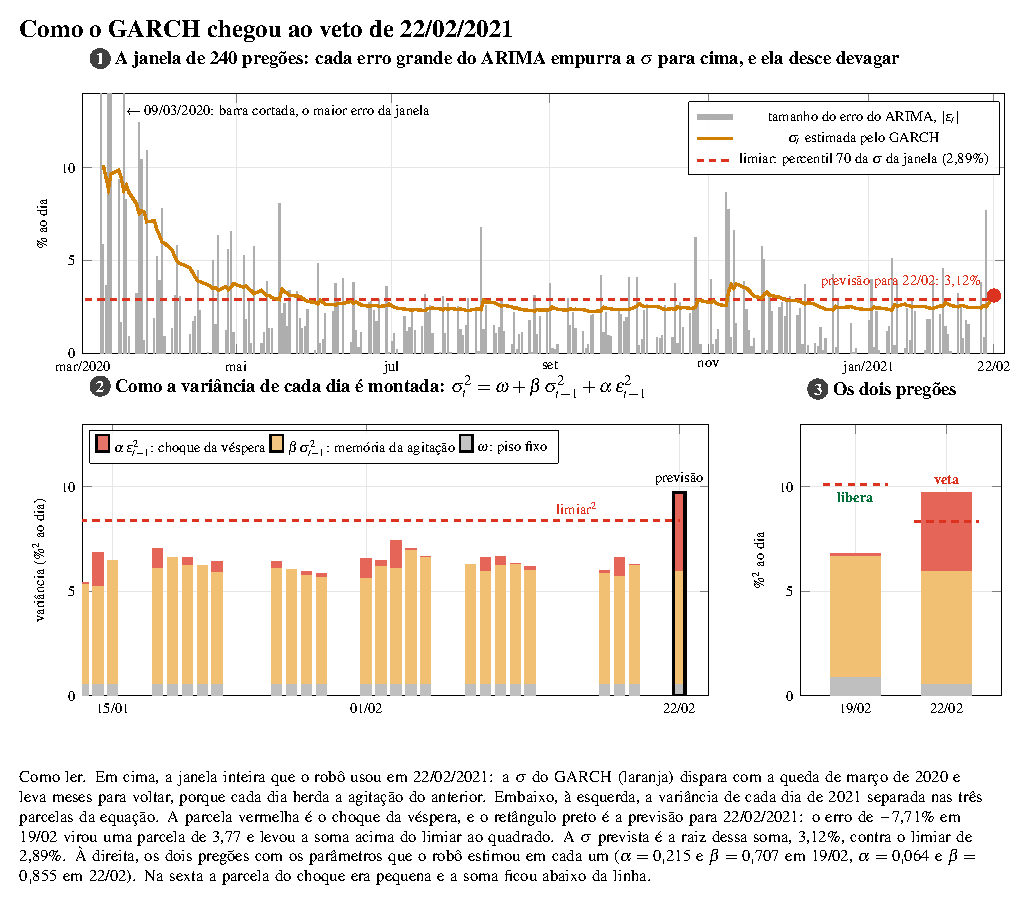
\includegraphics[width=\textwidth]{fig-garch.pdf}
\caption{O GARCH na janela do pregão de \vSegDia}
\label{fig:garch}
\end{figure}

\section{A equação em palavras}

O GARCH(1,1) do robô calcula a variância de cada dia como a soma de três parcelas:
\[
\sigma^2_t \;=\; \underbrace{\omega}_{\text{piso fixo}} \;+\; \underbrace{\beta\,\sigma^2_{t-1}}_{\text{memória}}
\;+\; \underbrace{\alpha\,\varepsilon^2_{t-1}}_{\text{choque da véspera}}
\]
O $\varepsilon$ é o erro do ARIMA, a diferença entre o retorno que aconteceu e o que ele previa. A parcela $\alpha\,\varepsilon^2$
é a reação: um erro grande ontem, para cima ou para baixo, aumenta a variância de hoje. A parcela $\beta\,\sigma^2$ é a
memória: um dia agitado deixa o seguinte agitado também, e a agitação vai se apagando aos poucos. O $\omega$ é o piso que
impede a variância de ir a zero. A volatilidade prevista é a raiz da soma, e o robô a compara com o limiar.

\section{Como ler a figura}

\begin{ideia}[Painel 1: a janela inteira]
As barras cinza são o tamanho do erro do ARIMA em cada dia dos 240 pregões que o robô usou. A linha laranja é a $\sigma$
que o GARCH atribui a cada um desses dias. Ela sobe quando chegam erros grandes e desce devagar depois, e é isso que
``memória'' quer dizer. A janela começa na queda de março de 2020, e a linha leva meses para voltar ao nível de
antes. O tracejado vermelho é o limiar, o percentil 70 dessa mesma linha, \vSegLim\%. O ponto vermelho é a previsão
para \vSegDia, \vSegVol\%, acima dele.
\end{ideia}

\begin{ideia}[Painel 2: a variância montada dia a dia]
Cada barra é a variância de um dia de 2021, separada nas três parcelas da equação. A cinza (piso) é igual em todas. A
laranja (memória) muda pouco de um dia para o outro. A vermelha (choque da véspera) é a que pula: quase some nos dias
calmos e cresce depois de um erro grande. O retângulo preto é a previsão para \vSegDia. O erro de \vSegUltRes\% em 19/02
virou uma parcela de \vSegPAlfa{} (em \%$^2$), e a soma, \vSegVarPrev, passou da linha do limiar ao quadrado. Sem essa
parcela, a barra ficaria abaixo da linha, como as anteriores.
\end{ideia}

\begin{ideia}[Painel 3: a sexta e a segunda]
São as previsões dos dois pregões seguidos, cada uma com os parâmetros estimados naquele dia. Na sexta, 19/02, a parcela do
choque era pequena (o erro da véspera tinha sido pequeno), a soma ficou em \vSexVarPrev{} contra uma linha mais alta, e o
GARCH liberou a compra. Na segunda, 22/02, o choque da sexta entrou na conta e o GARCH vetou.
\end{ideia}

\section{Cuidados}

\begin{cuidado}[O que não dizer a partir desta figura]
O GARCH não previu a queda de 22/02. Ele reagiu à de 19/02, que já tinha acontecido, e que o robô perdeu porque estava
comprado. O GARCH também não diz a direção: o erro de 19/02 pesaria o mesmo se fosse uma alta do mesmo tamanho, porque entra ao
quadrado.

A linha laranja do painel~1 é a $\sigma$ recalculada para toda a janela com os parâmetros estimados em \vSegDia. Não é a
sequência das previsões que o robô fez em cada um daqueles dias, porque a cada pregão ele reestima tudo. Essa sequência
real está na figura 11 da apresentação.

O limiar é o percentil 70 da própria linha laranja. Por construção, uns 30\% dos dias da janela ficam acima dele, e a
janela deste pregão inclui a crise de 2020 inteira, o que puxa o limiar para cima. A previsão, por sua vez, usa só o
último erro e a última variância, e por isso tende a ficar no topo da distribuição em fim de janela agitado (anotado no
\texttt{CLAUDE.md}, ``Semântica do limiar por percentil'').

Os parâmetros mudaram muito de um dia para o outro: $\alpha$ foi de \vSexAlfa{} para \vSegAlfa{} e $\beta$ de \vSexBeta{}
para \vSegBeta, com a janela andando um único pregão (saiu um dia de março de 2020 e entrou 19/02). A volatilidade
prevista subiu mesmo assim, porque o choque foi grande. Essa sensibilidade dos parâmetros não foi investigada aqui.
\end{cuidado}

\section{Procedência}

Os dados saem de \texttt{ferramentas/ModeloCompleto.mq5}, que roda as classes do próprio robô (\texttt{CArima},
\texttt{CGarch}, \texttt{Percentil}, \texttt{DecidirOperacao}) sobre os 240 fechamentos de \vSegIni{} a \vSegFim{} da
série \texttt{PETR4\_OFICIAL}. Previsão, volatilidade, limiar, veto, ordens e parâmetros coincidem com o traço gravado pelo
robô na refação de 05/10/2026. As três parcelas foram calculadas fora da classe \texttt{CGarch}, com os $\omega$, $\alpha$ e
$\beta$ dela, e a soma refeita bate com a $\sigma$ da classe (maior diferença da ordem de $10^{-17}$). Tudo está em
\texttt{dados/resultados/modelo\_completo\_2026-11-06/}.

Para refazer: \texttt{bash ferramentas/scripts/modelo\_completo.sh} e \texttt{make} nesta pasta.

\end{document}
